
\noindent This chapter covers the following ideas. 

\begin{enumerate}

\item Be able to use and understand matrix and vector notation, addition, scalar multiplication, the dot product, matrix multiplication, and matrix transposing. 
\item Use Gaussian elimination to solve systems of linear equations. Define and use the words homogeneous, nonhomogeneous, row echelon form, and reduced row echelon form. 
\item Find the rank of a matrix. Determine if a collection of vectors is linearly independent. If linearly dependent, be able to write vectors as linear combinations of the preceding vectors.
\item For square matrices, compute determinants, inverses, eigenvalues, and eigenvectors. 
\item Illustrate with examples how a nonzero determinant is equivalent to having independent columns, an inverse, and nonzero eigenvalues. Similarly a zero determinant is equivalent to having dependent columns, no inverse, and a zero eigenvalue. 

\end{enumerate}

The next unit will focus on applications of these ideas. The main goal of this unit is to familiarize yourself with the arithmetic involved in linear algebra.


\section{Basic Notation}
Most of linear algebra centers around understanding vectors, with matrices being functions which transform vectors from one vector space into vectors in another vector space. This chapter contains a brief introduction to the arithmetic involved with matrices and vectors.  The next chapter will show you many of the uses of the ideas we are learning. You will be given motivation for all of the ideas learned here, as well as real world applications of these ideas, before the end of the next chapter.  For now, I want you become familiar with the arithmetic of linear algebra so that we can discuss how all of the ideas in this chapter show up throughout the course.

\begin{definition}
\marginpar{
Matrix size is

row by column.} 
A matrix of size {$m$} by {$n$} has {$m$} rows and {$n$} columns.  We normally write matrices using capital letters, and use the notation 
$$A = 
\begin{bmatrix}
a_{11}&\cdots&a_{1n}\\ 
a_{21}&\cdots&a_{2n}\\ 
\vdots&\ddots&\vdots\\ 
a_{m1}&\cdots&a_{mn} 
\end{bmatrix} 
= [a_{jk}],$$
where $a_{jk}$ is the entry in the $j$th row, $k$th column. 
\begin{itemize}
 \item We say two matrices {$A$} and {$B$} are equal if {$a_{jk}=b_{jk}$} for all $j$ and $k$.
 \item We add and subtract matrices of the same size entry wise. So we write $A+B=C$ where $c_{jk} = a_{jk}+b_{jk}$. If matrices do not have the same size, then we cannot add them.
 \item We can multiply a matrix $A$ by a scalar $C$ to obtain a new matrix $cA$.  We do this multiplying every entry in the matrix $A$ by the scalar {$c$}.
 \item If the number of rows and columns are equal, then we say the matrix is square.  
 \item The main diagonal of a square ({$n \times n$}) matrix consists of the entries {$a_{11},a_{22},\ldots,a_{nn}$}. 
 \item The trace of a square matrix is the sum of the entries on the main diagonal ($\sum a_{jj}$). 
 \item The transpose of a matrix {$A=[a_{jk}]$} is a new matrix {$B=A^T$} formed by interchanging the rows and columns of $A$, so that $b_{jk}=a_{kj}$.  If $A^T=A$, then we say that $A$ is symmetric.
\end{itemize}
\end{definition}

\begin{problem}
Let $A=\begin{bmatrix}
1&3\\
0&2
\end{bmatrix}
$ and 
$B=
\begin{bmatrix}
3&-1\\
0&4
\end{bmatrix}
$.  
Compute $2A-3B$, and find the trace of both $A$ and $B$.  
\end{problem}


\begin{problem}
 Write down a 3 by 2 matrix, and compute the transpose of that matrix. Then give an example of a 3 by 2 symmetric matrix, or explain why it is not possible.
\end{problem}



Vectors represent a magnitude in a given direction. We can use vectors to model forces, acceleration, velocity, probabilities, electronic data, and more. We can use matrices to represent vectors. A row vector is a {$1\times n$} matrix. A column vector is an {$m \times 1$} matrix.   Textbooks often write vectors using bold face font. By hand (and in this book) we add an arrow above them. The notation ${\bf v} = \vec v = \left<v_1,v_2,v_3\right>$ can represent either row or column vectors. Many different ways to represent vectors are used throughout different books.  In particular, we can represent the vector $\left<2,3\right>$ in any of the following forms
$$\left<2,3\right>
= 2{\bf i}+3{\bf j} 
= (2,3) 
= \begin{bmatrix}2&3\end{bmatrix} 
= \begin{bmatrix}2\\3\end{bmatrix}
= \begin{pmatrix}2&3\end{pmatrix} 
= \begin{pmatrix}2\\3\end{pmatrix}
$$ 
The notation $(2,3)$ has other meanings as well (like a point in the plane, or an open interval), and so when you use the notation $(2,3)$, it should be clear from the context that you are working with a vector. 
{\marginpar{{
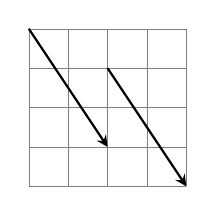
\begin{tikzpicture}[scale=.5]
\draw[help lines,step=1cm] (0,0) grid (4,4);
\draw[->,>=stealth,thick] (0,4) -- (2,1);
\draw[->,>=stealth,thick] [xshift=2cm, yshift=-1cm](0,4) -- (2,1);
\end{tikzpicture}

Both vectors 
represent $\left<2,-3\right>$, regardless of where we start.
}}}To draw a vector $\left<v_1,v_2\right>$, one option is to draw an arrow from the origin (the tail) to the point $(v_1,v_2)$ (the head). 
However, the tail does not have to be placed at the origin. 

The principles of addition and subtraction of matrices apply to vectors (which can be though of as row or column matrices). We will most often think of vectors as column vectors. 

\begin{definition}
The magnitude (or length) of the vector $\vec u = (u_1,u_2)$ is $|\vec u| = \sqrt{u_1^2+u_2^2}$.  In higher dimensions we extend this as $$\ds |\vec u| = \sqrt{u_1^2+u_2^2+u_3^2+\cdots u_n^2} = \sqrt{\sum_{i=1}^n u_i^2}.$$ 
A unit vector is a vector with length 1. 
\marginpar{A unit vector $\bf \hat u$ has length $|\vec u|=1$} 
In many books unit vectors are written with a hat above them, as $\bf{\hat u}$.
\end{definition}

We will need to be able to find vectors of any length that point in a given direction. 
\begin{problem}
 Find a vector of length $12$ that points in the same direction as the vector $\vec v = (1,2,3,4)$. Then give a general formula for finding a vector of length $c$ that points in the direction of $\vec u$. 
\end{problem}


The simplest vectors in 2D are a one unit increment in either the $x$ or $y$ direction, and we write these vectors in any of the equivalent forms 
$$\textbf{i} = \vec i = \left<1,0\right>=(1,0)\quad \text{and}\quad
  \textbf{j} = \vec j = \left<0,1\right>=(0,1).$$ 
We call these the standard basis vectors in 2D. 
In 3D we include the vector $\textbf{k} = \vec j=\left<0,0,1\right>$ as well as add a zero to both $\vec i$ and $\vec j$ to obtain the standard basis vectors. 
\marginpar{The standard basis vectors in 3D\\
$\textbf{i} = \vec i = \left<1,0,0\right>=(1,0,0)$\\   
$\textbf{j} = \vec j = \left<0,1,0\right>=(0,1,0)$\\ 
$\textbf{k} = \vec k = \left<0,0,1\right>=(0,0,1)$   
}
The word basis suggests that we can base other vectors on these basis vectors, and we typically write other vectors in terms of these standard basis vectors. 
Using only scalar multiplication and vector addition, we can obtain the other vectors in 2D from the standard basis vectors. 

\begin{problem}
 Write the vector $(2,3)$ in the form $(2,3) = c_1\vec i+c_2\vec j$.  

If instead we use the non-standard basis vectors $\vec u_1= (1,2)$ and $\vec u_2=(-1,4)$, then write the vector $(2,3)$ 
in the form $(2,3) = c_1\vec u_1+c_2\vec u_2$.
\end{problem}

\begin{definition}
A linear combination of vectors {$\vec v_{1},\vec v_{2},\ldots,\vec v_{n}$} is an expression of the form {$c_1\vec v_{1}+c_2\vec v_{2}+\ldots+c_n\vec v_{n}$}, where {$c_i$} is a constant for each $i$. 
\end{definition}

A linear combination of vectors is simply a sum of scalar multiples of the vectors. 
We start with some vectors, stretch each one by some scalar, and then sum the result. 
Much of what we will do this semester (and in many courses to come) relates directly to understanding linear combinations.  

\begin{problem}
 The force acting on an object is $\vec F = (-3,2)$ N. The object is in motion and has velocity vector $\vec v=(1,1)$ and acceleration vector $\vec a = (-1,2)$.  Write the force as a linear combination of the velocity and acceleration vectors. 
\end{problem}

\begin{problem}
 Write the vector $(2,3,1)$ as a linear combination of the standard basis vectors in $\mathbb{R}^3$.  Then write $(2,3,1)$ as a linear combination of the vectors $(1,0,0)$, $(1,1,0)$, and $(1,1,1)$.  
\end{problem}


One of the key applications of linear combinations we will make throughout the semester is matrix multiplication. Let's introduce the idea with an example.  
\begin{example}
Consider the three vectors 
$\begin{bmatrix}1\\0\\1\end{bmatrix}$,
$\begin{bmatrix}0\\2\\-3\end{bmatrix}$,
and 
$\begin{bmatrix}2\\1\\1\end{bmatrix}$.
Let's multiply the first vector by 2, the second by -1, and the third by 4, and then sum the result.  
This gives us the linear combination
$$2\begin{bmatrix}1\\0\\1\end{bmatrix}
-1\begin{bmatrix}0\\2\\-3\end{bmatrix}
+4\begin{bmatrix}2\\1\\1\end{bmatrix}
=
\begin{bmatrix}10\\2\\9\end{bmatrix} 
$$
We will define matrix multiplication so that multiplying a matrix on the right by a vector corresponds precisely to creating a linear combination of the columns of $A$. 
We now write the linear combination above in matrix form 
$$ 
\begin{bmatrix}1&0&2\\0&2&1\\1&-3&1\end{bmatrix}
\begin{bmatrix}2\\-1\\4\end{bmatrix}
=
\begin{bmatrix}10\\2\\9\end{bmatrix} 
.$$
\end{example}

\begin{definition}[A matrix times a vector]
We define the matrix product $A\vec x$ (a matrix times a vector) to be the linear combination of columns of $A$ where the components of $\vec x$ are the scalars in the linear combination. 
For this to make sense, notice that the vector $\vec x$ must have the same number of entries as there are columns in $A$. 
We can make this definition more precise as follows. 
Let $\vec v_i$ be the $i$th column of $A$ so that 
$A = \begin{bmatrix}\vec a_1 & \vec a_2 &\cdots &\vec a_n\end{bmatrix}$, 
and let $\vec x = \begin{bmatrix}x_1\\x_2\\ \hdots \\ x_n\end{bmatrix}$. Then the matrix product is the linear combination 
\marginpar{The product $A\vec x$ gives us linear combinations of the columns of $A$.}
$$A\vec x 
=\begin{bmatrix}\vec a_1 & \vec a_2 &\cdots &\vec a_n\end{bmatrix}\begin{bmatrix}x_1\\x_2\\ \hdots \\ x_n\end{bmatrix}
= \vec a_1 x_1+\vec a_2 x_2+\cdots +\vec a_n x_n.$$ 
\end{definition}
The definition above should look like the dot product. If you think of $A$ as a vector of vectors, then $A\vec x$ is just the dot product of $A$ and $\vec x$.  

\begin{problem}
 Write down a 2 by 4 nonzero matrix, and call it $A$ (fill the matrix with some integers of your choice). Then write down a vector $\vec x$ such that the matrix product $A\vec x$ makes sense (again, fill the vector with integers of your choice).  Then use the definition above to obtain the product $A\vec x$. 
\end{problem}


\begin{definition}[A matrix times a matrix]
Let $\vec b_j$ represent the $j$th column of $B$ (so $B = \begin{bmatrix}\vec b_1 & \vec b_2 &\cdots &\vec b_n\end{bmatrix}$).  The product $AB$ of two matrices {$A_{m\times n}$} and {$B_{n\times p}$} is a new matrix {$C_{m\times p}=[c_{ij}]$} where the $j$th column of $C$ is the product $A\vec b_j$.  To summarize, the matrix product $AB$ is a new matrix whose $j$th column is a linear combinations of the columns of $A$ using the entries of the $j$th column of $B$ to perform the linear combinations. 
\end{definition}


\begin{problem}
Let 
$A = 
\begin{bmatrix}
1&2\\
3&4\\
5&6
\end{bmatrix}
$ 
and
$B = 
\begin{bmatrix}
0&1&4\\
-1&2&-3
\end{bmatrix}
$.
Use the definition given above to compute both $AB$ and $BA$. Be prepared to show the class how you used linear combinations to get the matrix product.  (If you are used to using the row dotted by column approach, then this problem asks you to do the matrix product differently.)
\end{problem}

We introduced matrix multiplication in terms of linear combinations of column vectors. My hope is that by doing so you immediately start thinking of linear combinations whenever you encounter matrix multiplication (as this is what it was invented to do).  There are many alternate ways to think of matrix multiplication. Here are two additional methods. 
\begin{enumerate}
	\item ``Row times column approach.'' The product {$AB$} of two matrices {$A_{m\times n}$} and {$B_{n\times p}$} is a new matrix {$C_{m\times p}=[c_{ij}]$} where $c_{ij}=\sum_{k=1}^n a_{ik}b_{kj}$ is the dot product of the of the {$i$}th row of {$A$} and the {$j$}th column of B.  Wikipedia has an excellent visual illustration of this approach.	
	 
	\item Rephrase everything in terms of rows (instead of columns). We form linear combinations of rows using rows.  The matrix product $\vec x B$ (notice the order is flopped) is a linear combination of the rows of $B$ using the components of $x$ as the scalars. For the product $AB$, let $\vec a_i$ represent the $i$th row of $A$.  Then the $i$th row of $AB$ is the product $\vec a_iB$. We'll most often use the column definition instead of this, because we use the function notation $f(x)$ from calculus, and later we will use the notation $A(\vec x)$ instead of $(\vec x)A$ to describe how matrices act as functions. 
\end{enumerate}


\begin{problem}
Let 
$A = 
\begin{bmatrix}
1&2\\
3&4\\
5&6
\end{bmatrix}
$ 
and
$B = 
\begin{bmatrix}
0&1&4\\
-1&2&-3
\end{bmatrix}
$.
Use the two alternate definitions above to compute $AB$. Be prepared to show the class how you used both alternate definitions (You'll need to show your intermediate steps).
\end{problem}

\begin{problem}
Do each of the following:
\begin{enumerate}
 \item Solve the system of equations $x+2y=3$, $4x+5y=6$.
 \item Write the vector $\pvec{3\\6}$ as a linear combination of $\pvec{1\\4}$ and $\pvec{2\\5}$.
 \item Let $A = \pvec{1&2\\4&5}$ and $\vec b=\pvec{3\\6}$.  Find a vector $\vec x$ so that $A\vec x = \vec b$. This matrix $A$ is called the coefficient matrix of the system in the first part.  
\end{enumerate}
How are these three questions related?
 
\end{problem}

Prior to introducing Gaussian elimination, let's solve a system of equations using an elimination method.  If $2x+3y=4$ and $5x+7y=0$, then we can eliminate $x$ from the second equation by multiplying both sides of the first equation by 5, and both sides of the second equation by 2, and then subtracting.  This would give us the equations $10x+15y=20$ and $10x+14y=1$. The first equation minus the second then gives $(10-10)x+(15-14)y=(20-0)$, or more simply $y=20$. Similarly, you could multiply the first equation by 7, and the second by $3$, to eliminate $y$.  

\begin{problem}
 Solve the system of equations 
\begin{align*}
  2x+3y-4z&=4\\  
  3x+4y-3z&=8\\  
  7x+12y-12z&=19.  
\end{align*}
Use elimination to find your solution. Eliminate $x$ from the 2nd and 3rd equations (which will give you two equations that do not involve $x$). Then use one of these simplified equations to eliminate $y$ from the other simplified equation. At this point you should have an equation that only involves $z$. Then use back substitution to give $y$ and $x$.   
\end{problem}

\begin{problem}
Answer the following.
\begin{enumerate}
 \item Suppose that $ax+by=c$ and $dx+ey=f$, where $a,b,c,d,e,f$ are all constants.  This is a system of equations with 2 equations and 2 unknowns.  Each equation represents a line in the plane.  How many solutions are there to this system?  (You should have a few different cases.)
 \item Suppose that $a_{11}x+a_{12}y+a_{13}z=b_1$, $a_{21}x+a_{22}y+a_{23}z=b_2$ and $a_{31}x+a_{32}y+a_{33}z=b_1$, where each $a_{ij}$ is a constant. This is a system of equations with 3 equations and 3 unknowns.  Each equation represents a plane in space.  How many solutions are there to this system?  (You should have a few different cases.)
 \item Suppose that $a_{11}x+a_{12}y+a_{13}z=b_1$ and $a_{21}x+a_{22}y+a_{23}z=b_2$, where each $a_{ij}$ is a constant. This is a system of equations with 2 equations and 3 unknowns.  Each equation represents a plane in space.  How many solutions are there to this system?  (You should have a few different cases.)
\end{enumerate}
\end{problem}

\begin{definition}
 We say that a system of linear equation is consistent, if it has at least one solution.  We say it is inconsistent if there is no solution. 
\end{definition}

\section{Gaussian Elimination}
Gaussian elimination is an efficient algorithm we will use to solve systems of equations. This is the same algorithm implemented on most computers systems. The main idea is to eliminate each variable from all but one equation/row (if possible), using the following three operations (called elementary row operations):
\begin{enumerate}
  \item Multiply an equation (or row of a matrix) by a nonzero constant,
  \item Add a nonzero multiple of any equation (or row) to another equation,
  \item Interchange two equations (or rows).
\end{enumerate}
These three operations are the operations learned in college algebra when solving a system using a method of elimination.  Gaussian elimination streamlines elimination methods to solve generic systems of equations of any size. The process involves a forward reduction and (optionally) a backward reduction. The forward reduction creates zeros in the lower left corner of the matrix.  The backward reduction puts zeros in the upper right corner of the matrix. We eliminate the variables in the lower left corner of the matrix, starting with column 1, then column 2, and proceed column by column until all variables which can be eliminated (made zero) have been eliminated. Before formally stating the algorithm, let's look at a few examples. 

\begin{example}
Let's start with a system of 2 equations and 2 unknowns. I will write the augmented matrix representing the system as we proceed. To solve $$
\begin{array}{rr}
\begin{array}{rl}
x_1-3x_2&=4\\
2x_1-5x_2&=1 
\end{array}
&
\begin{bmatrix}[cc|c] 1&-3&4\\2&-5&1
\end{bmatrix} 
\end{array}
$$
we eliminate the $2x_1$ in the 2nd row by adding -2 times the first row to the second row.
$$\begin{array}{rr}
\begin{array}{rl}
x_1-3x_2&=4\\
x_2&=-7 
\end{array}
&
\begin{bmatrix}[cc|c] 1&-3&4\\0&1&-7
\end{bmatrix} 
\end{array}
$$
The matrix at the right is said to be in \textbf{row echelon form}. \marginpar{row echelon form} 
\begin{definition}[Row Echelon Form]
We say a matrix is in row echelon form (ref) if
\begin{itemize}
  \item each nonzero row begins with a 1 (called a leading 1),
  \item the leading 1 in a row occurs further right than a leading 1 in the row above, and
  \item any rows of all zeros appear at the bottom.
\end{itemize}
The position in the matrix where the leading 1 occurs is called a pivot. 
The column containing a pivot is called a pivot column. \marginpar{pivot column}
\end{definition}
At this point in our example, we can use ``back-substitution'' to get {$x_2=-7$} and {$x_1=4+3x_2 = 4-21=-17$}. 
Alternatively, we can continue the elimination process by eliminating the terms above each pivot, starting on the right and working backwards. 
This will result in a matrix where all the pivot columns contain all zeros except for the pivot. 
If we add 3 times the second row to the first row, we obtain.
$$\begin{array}{rr}
\begin{array}{rl}
x_1&=-17\\
x_2&=-7 
\end{array}
&
\begin{bmatrix}[cc|c] 1&0&-17\\0&1&-7
\end{bmatrix} 
\end{array}
$$
The matrix on the right is said to be in \textbf{reduced row echelon form} (or just rref). 
We can easily read solutions to systems of equations directly from a matrix which is in reduced row echelon form.

\begin{definition}[Reduced Row Echelon Form]
\marginpar{reduced row echelon form - rref}
We say that a matrix is in reduced row echelon form (rref) if 
\begin{itemize}
\item the matrix is in row echelon form, and 
\item each pivot column contains all zeros except for the pivot (leading one).
\end{itemize}
\end{definition}


\end{example}


\begin{example}
Let's now solve a nonhomogeneous (meaning the right side is not zero) system with 3 equations and 3 unknowns: $$\begin{array}{rl}
2x_1+x_2-x_3&=2\\
x_1-2x_2 &=3\\
4x_2+2x_3&=1
\end{array} \quad\quad\quad\quad\quad
 \begin{bmatrix}[ccc|c] 2&1&-1&2\\1&-2&0&3\\0&4&2&1\end{bmatrix}.$$ 
We'll encounter some homogeneous systems later on.
To simplify the writing, we'll just use matrices this time. 
To keep track of each step, I will write the row operation next to the row I will replace. 
Remember that the 3 operations are (1)multiply a row by a nonzero constant, (2)add a multiple of one row to another, (3) interchange any two rows.  
If I write $R_2+3R1$ next to $R_2$, then this means I will add 3 times row 1 to row 2.  
If I write $2R_2-R1$ next to $R_2$, then I have done two row operations, namely I multiplied $R_2$ by 2, and then added (-1) times $R1$ to the result (replacing $R2$ with the sum). 
The steps below read left to right, top to bottom. 
In order to avoid fractions, I wait to divide until the last step, only putting a 1 in each pivot at the very end.
$$\begin{array}{rlcl}
\Rightarrow^{(1)}&
 \begin{bmatrix}[ccc|c] 2&1&-1&2\\1&-2&0&3\\0&4&2&1\end{bmatrix}
  \begin{array}{lr} \ \\2R_2-R_1\\ \ \end{array}
&\Rightarrow^{(2)}& 
\begin{bmatrix}[ccc|c] 2&1&-1&2\\0&-5&1&4\\0&4&2&1\end{bmatrix} 
\begin{array}{lr}\ \\ \ \\5R_3+4R_2 \end{array}
\\ \\ \Rightarrow^{(3)}&
 \begin{bmatrix}[ccc|c] 2&1&-1&2\\0&-5&1&4\\0&0&14&21\end{bmatrix} 
 \begin{array}{lr}\ \\ \ \\R_3/7 \end{array}
&\Rightarrow^{(4)}& 
\begin{bmatrix}[ccc|c] 2&1&-1&2\\0&-10&2&8\\0&0&2&3\end{bmatrix} 
\begin{array}{l} 2R_1+R_3\\R_2-R_3\\ \ \end{array}
\\ \\ \Rightarrow^{(5)}&
 \begin{bmatrix}[ccc|c] 4&2&0&7\\0&-10&0&5\\0&0&2&3\end{bmatrix}  
 \begin{array}{lr}\ \\R_2/5\\ \ \end{array} 
&\Rightarrow^{(6)}& 
\begin{bmatrix}[ccc|c] 4&2&0&7\\0&-2&0&1\\0&0&2&3\end{bmatrix}  
\begin{array}{lr} R_1+R_2\\ \ \\ \ \end{array}
\\ \\ \Rightarrow^{(7)}&
\begin{bmatrix}[ccc|c] 4&0&0&8\\0&-2&0&1\\0&0&2&3\end{bmatrix} 
\begin{array}{lr} R_1/4\\R_2/-2\\R_3/2 \end{array}
&\Rightarrow^{(8)}&  
\begin{bmatrix}[ccc|c] 1&0&0&2\\0&1&0&-1/2\\0&0&1&3/2\end{bmatrix} 
\end{array}
$$
Writing the final matrix in terms of a system, we have the solution {$x_1=2, x_2=-1/2, x_3=3/2$}. Remember that this tells us (1) where three planes intersect, (2) how to write the 4th column $\vec b$ in our original augmented matrix as a linear combination of the columns of the coefficient matrix $A$, and (3) how to solve the matrix equation $A\vec x = \vec b$ for $\vec x$.
\end{example}


The following steps describe the Gaussian elimination algorithm that we used above. 
Please take a moment to compare what is written below with the example above. 
Most of the problems in this unit can be solved using Gaussian elimination, so we will practice it as we learn a few new ideas.
\begin{enumerate}
\item Forward Phase (row echelon form) - The following 4 steps should be repeated until you have mentally erased all the rows or all the columns. In step 1 or 4 you will erase a column and/or row from the matrix.
\begin{enumerate}
	\item  
	\marginpar{Computer algorithms place the largest (in absolute value) nonzero entry in the first row. This reduces potential errors due to rounding that can occur in later steps.}
Consider the first column of your matrix. Start by interchanging rows (if needed) to place a nonzero entry in the first row. If all the elements in the first column are zero, then ignore that column in future computations (mentally erase the column) and begin again with the smaller matrix which is missing this column. If you erase the last column, then stop.
  \item 
  Divide the first row (of your possibly smaller matrix) row by its leading entry so that you have a leading 1. This entry is a pivot, and the column is a pivot column. [When doing this by hand, it is often convenient to skip this step and do it at the very end so that you avoid fractional arithmetic. If you can find a common multiple of all the terms in this row, then divide by it to reduce the size of your computations.  ] 
	\item Use the pivot to eliminate each nonzero entry below the pivot, by adding a multiple of the top row (of your smaller matrix) to the nonzero lower row.
	\item 
	\marginpar{Ignoring rows and columns is equivalent to incrementing row and column counters in a computer program.}
	Ignore the row and column containing your new pivot and return to the first step (mentally cover up or erase the row and column containing your pivot). If you erase the last row, then stop.
\end{enumerate}
	\item Backward Phase (reduced row echelon form - often called Gauss-Jordan elimination) - At this point each row should have a leading 1, and you should have all zeros to the left and below each leading 1. If you skipped step 2 above, then at the end of this phase you should divide each row by its leading coefficient to make each row have a leading 1.
\begin{enumerate}
	\item Starting with the last pivot column. Use the pivot in that column to eliminate all the nonzero entries above it, by adding multiples of the row containing the pivot to the nonzero rows above. 
	\item Work from right to left, using each pivot to eliminate the nonzero entries above it. Nothing to the left of the current pivot column changes.  By working right to left, you greatly reduce the number of computations needed to fully reduce the matrix.
\end{enumerate}
\end{enumerate}


\begin{example}\label{ex rref last}
As a final example, let's reduce 
{\small $
\begin{bmatrix}[cccc|c]
 0 & 1 & 1 & -2 & 7 \\
  1 & 3 & 5 & 1 & 6 \\
 2 & 0 & 4 & 3 & -8 \\
 -2 & 1 & -3 & 0 & 5
\end{bmatrix}
$} to reduced row echelon form (rref). The first step involves swapping 2 rows. We swap row 1 and row 2 because this places a 1 as the leading entry in row 1.
{\small  $$\begin{array}{rlcl}
\multicolumn{2}{l}{\text{(1) Get a nonzero entry in upper left}}&
\multicolumn{2}{l}{\text{(2) Eliminate entries in 1st column}}\\
\Rightarrow&
\begin{bmatrix}[cccc|c]
 0 & 1 & 1 & -2 & 7 \\
  1 & 3 & 5 & 1 & 6 \\
 2 & 0 & 4 & 3 & -8 \\
 -2 & 1 & -3 & 0 & 5
\end{bmatrix}
  \begin{array}{lr} R_1\leftrightarrow R_2 \\ \ \\ \ \\ \ \end{array}
&\Rightarrow& 
\begin{bmatrix}[cccc|c]
  1 & 3 & 5 & 1 & 6 \\
 0 & 1 & 1 & -2 & 7 \\
 2 & 0 & 4 & 3 & -8 \\
 -2 & 1 & -3 & 0 & 5
\end{bmatrix}
  \begin{array}{lr} \ \\ \ \\ R_3-2R_1 \\ R_4+2R_1 \end{array}
\\ \\
\multicolumn{2}{l}{\text{(3) Eliminate entries in 2nd column}}&
\multicolumn{2}{l}{\text{(4) Make a leading 1 in 4th column}}\\
\Rightarrow&
\begin{bmatrix}[cccc|c]
  1 & 3 & 5 & 1 & 6 \\
 0 & 1 & 1 & -2 & 7 \\
 0 & -6 & -6 & 1 & -20 \\
 0 & 7 & 7 & 2 & 17
\end{bmatrix}
  \begin{array}{lr} \ \\ \ \\ R_3+6R_2 \\ R_4-7R_2 \end{array}
&\Rightarrow& 
\begin{bmatrix}[cccc|c]
  1 & 3 & 5 & 1 & 6 \\
 0 & 1 & 1 & -2 & 7 \\
 0 & 0 & 0 & -11 & 22 \\
 0 & 0 & 0 & 16 & -32
\end{bmatrix}
  \begin{array}{lr} \ \\ \ \\ R_3/(-11) \\ R_4/16 \end{array}
\\ \\
\multicolumn{2}{l}{\text{(5) Eliminate entries in 4th column}}&
\multicolumn{2}{l}{\text{(6) Row Echelon Form}}\\
\Rightarrow&
\begin{bmatrix}[cccc|c]
  1 & 3 & 5 & 1 & 6 \\
 0 & 1 & 1 & -2 & 7 \\
 0 & 0 & 0 & 1 & -2 \\
 0 & 0 & 0 & 1 & -2
\end{bmatrix}
  \begin{array}{lr} \ \\ \ \\ \ \\ R_4-R_3 \end{array}
&\Rightarrow& 
\begin{bmatrix}[cccc|c]
  1 & 3 & 5 & 1 & 6 \\
 0 & 1 & 1 & -2 & 7 \\
 0 & 0 & 0 & 1 & -2 \\
 0 & 0 & 0 & 0 & 0
\end{bmatrix}
\end{array}
$$}\begin{picture}(0,0)

\begin{tikzpicture}[scale=.39]
\draw[help lines,step=1cm,transparent] (0,0) grid (30,20);
\draw[opacity=.2,fill][shift={(2.6,16.6)}] (0,0) rectangle (1.4,.8);
\draw[opacity=.2,fill][shift={(19.6,13.6)}] (0,0) rectangle (1.4,2.8);
\draw[opacity=.1,fill][shift={(2.6,10.6)}] (0,0) rectangle (8.9,.8);
\draw[opacity=.1,fill][shift={(2.6,7.6)}] (0,0) rectangle (.7,3.8);
\draw[opacity=.2,fill][shift={(3.9,7.6)}] (0,0) rectangle (1.4,1.8);
\draw[opacity=.1,fill][shift={(19.5,10.6)}] (0,0) rectangle (8.1,.8);
\draw[opacity=.1,fill][shift={(19.5,7.6)}] (0,0) rectangle (.7,3.8);
\draw[opacity=.1,fill][shift={(20.8,9.6)}] (0,0) rectangle (6.8,.8);
\draw[opacity=.1,fill][shift={(20.8,7.6)}] (0,0) rectangle (.7,2.8);
\draw[opacity=.1,fill][shift={(22.15,7.6)}] (0,0) rectangle (.7,1.8);
\draw[opacity=.2,fill][shift={(23.6,8.6)}] (0,0) rectangle (1.6,.8);

\draw[opacity=.1,fill][shift={(2.6,4.6)}] (0,0) rectangle (7.2,.8);
\draw[opacity=.1,fill][shift={(2.6,1.6)}] (0,0) rectangle (.7,3.8);
\draw[opacity=.1,fill][shift={(3.9,3.6)}] (0,0) rectangle (5.9,.8);
\draw[opacity=.1,fill][shift={(3.9,1.6)}] (0,0) rectangle (.7,2.8);
\draw[opacity=.1,fill][shift={(5.2,1.6)}] (0,0) rectangle (.7,1.8);
\draw[opacity=.2,fill][shift={(6.7,1.6)}] (0,0) rectangle (1.1,.8);

\draw[opacity=.1,fill][shift={(19.5,4.6)}] (0,0) rectangle (7.2,.8);
\draw[opacity=.1,fill][shift={(19.5,1.6)}] (0,0) rectangle (.7,3.8);
\draw[opacity=.1,fill][shift={(20.8,3.6)}] (0,0) rectangle (5.9,.8);
\draw[opacity=.1,fill][shift={(20.8,1.6)}] (0,0) rectangle (.7,2.8);
\draw[opacity=.1,fill][shift={(22.15,1.6)}] (0,0) rectangle (.7,1.8);
\draw[opacity=.1,fill][shift={(23.6,1.6)}] (0,0) rectangle (1.1,1.8);
\draw[opacity=.1,fill][shift={(23.6,2.6)}] (0,0) rectangle (3.1,.8);
\draw[opacity=.1,fill][shift={(25.6,1.6)}] (0,0) rectangle (1.1,.8);

\end{tikzpicture}
\end{picture}At this stage we have found a row echelon form of the matrix. 
Notice that we eliminated nonzero terms in the lower left of the matrix by starting with the first column and working our way over column by column.  Columns 1, 2, and 4 are the pivot columns of this matrix. We now use the pivots to eliminate the other nonzero entries in each pivot column (working right to left).\marginpar{Recall that a matrix is in reduced row echelon (rref) if:
\begin{enumerate}
	\item Nonzero rows begin with a leading 1. 
	\item Leadings 1's on subsequent rows appear further right than previous rows. 
	\item Rows of zeros are at the bottom.
	\item Zeros are above and below each pivot.
\end{enumerate}}
{\small $$ \begin{array}{rlcl}
\multicolumn{2}{l}{\text{(7) Eliminate entries in 4th column}}&
\multicolumn{2}{l}{\text{(8) Eliminate entries in 2nd column}}\\
\Rightarrow&
\begin{bmatrix}[cccc|c]
  1 & 3 & 5 & 1 & 6 \\
 0 & 1 & 1 & \begin{picture}(0,0)(0,3) \tikz \draw[scale=.39,fill,opacity=.2] (0,0) rectangle (1.6,2);\end{picture}
							-2 & 7 \\
 0 & 0 & 0 & 1 & -2 \\
 0 & 0 & 0 & 0 & 0
\end{bmatrix}
  \begin{array}{lr} R_1-R3 \\ R_2+2R_3 \\ \ \\ \ \end{array}
&\Rightarrow& 
\begin{bmatrix}[cccc|c]
  1 & \begin{picture}(0,0)(4,3) \tikz \draw[scale=.39,fill,opacity=.2] (0,0) rectangle (1,1);\end{picture}
  		3 & 5 & 0 & 8 \\
 0 & 1 & 1 & 0 & 3 \\
 0 & 0 & 0 & 1 & -2 \\
 0 & 0 & 0 & 0 & 0
\end{bmatrix}
  \begin{array}{lr} R_1-3R_2 \\ \ \\ \ \\ \ \end{array}
\\ \\ 
\multicolumn{2}{l}{\text{(9) Reduced Row Echelon Form}}&
\multicolumn{2}{l}{\text{(10) Switch to system form}}\\
\Rightarrow&
\begin{bmatrix}[cccc|c]
  1 & 0 & 2 & 0 & -1 \\
 0 & 1 & 1 & 0 & 3 \\
 0 & 0 & 0 & 1 & -2 \\
 0 & 0 & 0 & 0 & 0
\end{bmatrix}
&\Rightarrow& 
\begin{array}{rl}
x_1+2x_3&=-1\\
x_2+x_3&=3\\
x_4&=-2\\
0&=0
\end{array}
\end{array}
$$}We have obtained the reduced row echelon form. 
When we write this matrix in the corresponding system form, notice that there is not a unique solution to the system. Because the third column did not contain a pivot column, we can write every variable in terms of $x_3$ (the redundant equation $x_3=x_3$ allows us to write $x_3$ in terms of $x_3$). We are free to pick any value we want for $x_3$ and still obtain a solution. For this reason, we call $x_3$ a free variable, \marginpar{Free variables correspond to non pivot columns. Solutions can be written in terms of free variables.} and write our infinitely many solutions in terms of $x_3$ as 
$$
\begin{array}{ll}
x_1=-1-2x_3\\
x_2=3-x_3\\
x_3=x_3\\
x_4=-2
\end{array}
\quad \text{ or by letting $x_3=t$ }\quad
\begin{array}{ll}
x_1=-1-2t\\
x_2=3-t\\
x_3=t\\
x_4=-2
\end{array}
.
$$
\marginpar{parametric form}By choosing a value (such as $t$) for $x_3$, we can write our solution in so called parametric form. We have now given a parametrization of the solution set, where $t$ is an arbitrary real number. 
\end{example}




\begin{problem}
Each of the following augmented matrices requires one row operation to be in reduced row echelon form. Perform the required row operation, and then write the solution to the corresponding system of equations in terms of the free variables.
\begin{multicols}{2}
\begin{enumerate}
	\item 
$
\begin{bmatrix}[ccc|c]
 1 & 0 & 0 & 3 \\
 0 & 0 & 1 & 1 \\
 0 & 1 & 0 & -2
\end{bmatrix}
$
	\item 
$
\begin{bmatrix}[ccc|c]
 1 & 2 & 0 & -4 \\
 0 & 0 & 1 & 3 \\
 -3 & -6 & 0 & 12
\end{bmatrix}
$
	\item 
$
\begin{bmatrix}[ccc|c]
 1 & 0 & 2 & 4 \\
 0 & 1 & -3 & 0 \\
 0 & 0 & 0 & 1
\end{bmatrix}
$
	\item 
$
\begin{bmatrix}[ccccc|c]
 0 & 1 & 0 & 7 & 0 & 3 \\
 0 & 0 & 1 & 5 & -3 & -10 \\
 0 & 0 & 0 & 0 & 1 & 2 \\
 0 & 0 & 0 & 0 & 0 & 0
\end{bmatrix}
$
\end{enumerate}
\end{multicols}
\end{problem}

\begin{problem}
Use Gaussian elimination to solve 
 $$
\begin{array}{rl}
  x_2 -2x_3 &= -5 \\
 2x_1 -x_2 + 3x_3 &= 4 \\
 4x_1 +x_2 + 4x_3 &= 5
\end{array}
$$
by row reducing the matrix to reduced row echelon form.
[Hint: Start by interchanging row 1 and row 2.] 
\end{problem}

\begin{problem}
Use Gaussian elimination to solve 
 $$
\begin{array}{rl}
 x_1 -2x_2 +x_3 &= 4 \\
 -x_1 + 2x_2 + 3x_3 &= 8 \\
 2x_1  -4x_2 +x_3 &= 5
\end{array}
$$
by row reducing the matrix to reduced row echelon form.
[Hint: You should end up with infinitely many solutions. State your solution by writing each variable in terms of the free variable(s).]
\end{problem}

\begin{problem}
Use Gaussian elimination to solve 
 $$
\begin{array}{rl}
 x_1 + 2x_3 + 3x_4 &= -7 \\
 2x_1 +x_2 + 4x_4 &= -7 \\
 -x_1 + 2x_2 + 3x_3  &= 0 \\
 x_2  -2x_3  -x_4 &= 4
\end{array}
$$
by row reducing the matrix to reduced row echelon form.

\end{problem}




\section{Rank, Linear Independence, Inverses, and Determinants}

\begin{definition}
\begin{itemize}
 \item The rank of a matrix is the number of pivot columns of the matrix. To find the rank of a matrix, you reduce the matrix using Gaussian elimination until you discover the pivot columns.
 \item The span of a set of vectors $\{\vec v_1,\vec v_2, \ldots, \vec v_n\}$ is all possible linear combinations of the vectors. In terms of matrices, the span of a set of vectors is all possible vectors $\vec b$ such that $A\vec x=\vec b$ for some vector $\vec x$, where the vectors $\vec v_i$ are placed in the columns of $A$.
 \item We say that a set of vectors $\{\vec v_1,\vec v_2, \ldots, \vec v_n\}$ is linearly independent if the only solution to the homogeneous system $c_1\vec v_{1}+c_2\vec v_{2}+\ldots+c_n\vec v_{n}=\vec 0$ is the trivial solution $c_1=c_2=\cdots=c_n=0$. 
Otherwise we say the vectors are linearly dependent, and it is possible to write one of the vectors as a linear combination of the others. 
We say the vectors are dependent because one of them depends on (can be obtained as a linear combination of) the others. 
 \item In terms of spans, we say vectors are linearly dependent when one of them is in the span of the other vectors. 
\end{itemize}
\end{definition}

As we complete each of the following problems in class, we'll talk about the span of the vectors, and the rank of the corresponding matrix.  The key thing we need to focus on is learning to use the words ``linearly independent'' and ``linearly dependent.''

\begin{problem}
 Are the vectors $\vec v_1 = (1,3,5)$, $ \vec v_2=(-1,0,1)$, and $\vec v_3=(0,3,1)$ linearly independent?  Solve the system $c_1\vec v_1+c_2\vec v_2+c_3\vec v_3=\vec 0$ to answer this question. If they are dependent, then write one of the vectors as a linear combination of the others.
\end{problem}


\begin{problem}
 Are the vectors $\vec v_1 = (1,2,0)$, $ \vec v_2=(2,0,3)$, and $\vec v_3=(3,-2,6)$ linearly independent?  Solve the system $c_1\vec v_1+c_2\vec v_2+c_3\vec v_3=\vec 0$ to answer this question.  If they are dependent, then write one of the vectors as a linear combination of the others. 
\end{problem}

 

\begin{problem}
Answer each of the following:
\begin{enumerate}
 \item  Suppose you have row reduced a 3 by 3 matrix, and discovered that the rank of the matrix is 2.  Are the columns of the matrix independent or dependent?  What if the rank was 3?  

 \item Now suppose you have row reduced a 7 by 7 matrix. If the columns are independent, what possible options do you have for the rank.

 \item Now suppose you have row reduced a 7 by 5 matrix. If the columns are independent, what must the rank be.

 \item Now suppose you have row reduced a 5 by 7 matrix. Explain why the columns cannot be independent. 

 \item If you have $n$ vectors placed in the columns of a matrix, what must the rank of the matrix be in order to guarantee that the vectors are independent?

\end{enumerate}

\end{problem}


\begin{problem}
 Is the vector $[2, 0, 1, -5]$ in the span of $$\{[1, 0, -1, -2], [1, 2, 3, 0], [0, 1, -1, 2]\}?$$ If it is, then write it as a linear combination of the others.  If it is not, then explain why it is not.
\end{problem}






\begin{problem}
Find the reduced row echelon form of the matrix
$$
B = 
\begin{bmatrix}
\nvec{2\\1}&
\nvec{-1\\1}&
\nvec{1\\0}&
\nvec{0\\1}&
\nvec{2\\0}&
\nvec{0\\3}&
\nvec{2\\3}
\end{bmatrix}.
$$
Use your result to answer the following questions.
\begin{enumerate}
 \item Write both $(1,0)$ and $(0,1)$ as linear combinations of $(2, 1)$ and $(-1,1)$. 
 \item Write  $\pvec{2\\0}$ as a linear combination of $\pvec{2\\1}$ and $\pvec{-1\\1}$.  Then write $\pvec{8\\0}$ as a linear combination of $\pvec{2\\1}$ and $\pvec{-1\\1}$. 
 \item Let $A = \begin{bmatrix}\nvec{2\\1}&\nvec{-1\\1}\end{bmatrix}$.  Find vectors $\vec x$ and $\vec y$ so that 
 $A\vec x = \pvec{1\\0}$ and $A\vec y = \pvec{0\\1}$.
 \item Find a matrix $B$ so that $AB = \begin{bmatrix}\nvec{1\\0}&\nvec{0\\1}\end{bmatrix}$. 
\end{enumerate}
 
\end{problem}

\begin{problem*}[21, revised]
Answer each of the following questions.
\begin{enumerate}
\item Find the reduced row echelon form of the matrix
$$
B = 
\begin{bmatrix}
\nvec{2\\1}&
\nvec{-1\\1}&
\nvec{1\\0}&
\nvec{0\\1}&
\nvec{2\\0}&
\nvec{0\\3}&
\nvec{2\\3}
\end{bmatrix}.
$$
 \item Write $(1,0)$ as a linear combination of $(2, 1)$ and $(-1,1)$. Remember, that when writing $c_1(2,1)+c_2(-1,1)=(1,0)$, you must solve for the unknown constants. Feel free to row reduce the augmented matrix  
$\begin{bmatrix}
\nvec{2\\1}&
\nvec{-1\\1}&
\nvec{1\\0}
\end{bmatrix}.
$
 \item Write $(0,1)$ as a linear combination of $(2, 1)$ and $(-1,1)$. Remember, that when writing $c_1(2,1)+c_2(-1,1)=(0,1)$, you must solve for the unknown constants. Feel free to row reduce the augmented matrix  
$\begin{bmatrix}
\nvec{2\\1}&
\nvec{-1\\1}&
\nvec{0\\1}
\end{bmatrix}
$. 
 \item Continue to write each of $\pvec{2\\0}$, $\pvec{0\\3}$, and $\pvec{2\\3}$ as a linear combination of $\pvec{2\\1}$ and $\pvec{-1\\1}$. [Hint:At some point, rather than row reducing 
$\begin{bmatrix}
\nvec{2\\1}&
\nvec{-1\\1}&
\vec v
\end{bmatrix}
$, ask yourself how you could use part 1 to answer this.]
\item The following matrix row reduces to give
$$\begin{bmatrix}
1 & 0 & 2 & 4 & 5 & 8 \\
0 & 2 & 5 & 2 & -1 & 3 \\
0 & -2 & -1 & 0 & 2 & 1
\end{bmatrix}
\xrightarrow{\text{rref}}
\begin{bmatrix}
1 & 0 & 0 & 3 & \frac{9}{2} & 6 \\
0 & 1 & 0 & -\frac{1}{4} & -\frac{9}{8} & -1 \\
0 & 0 & 1 & \frac{1}{2} & \frac{1}{4} & 1 
\end{bmatrix}
.$$
Use this to write both $(4,2,0)$ and $(5,-1,2)$ as a linear combination of the first three columns.
\end{enumerate}
 
\end{problem*}

\begin{definition}
 The identity matrix $I$ is a square matrix so that if $A$ is a square matrix, then $IA=AI=A$. The identity matrix acts like the number 1 when performing matrix multiplication.

 If $A$ is a square matrix, then the inverse of $A$ is a matrix $A^{-1}$ where we have $AA^{-1}=A^{-1}A=I$, provided such a matrix exists.
\end{definition}



\begin{problem*}
Let 
$A=
\begin{bmatrix}
\nvec{1\\3}&
\nvec{3\\4}
\end{bmatrix}
.$
We now develop an algorithm for computing the inverse $A^{-1}$.
If an inverse matrix exists, then we know it's the same size as $A$, so we could let $A^{-1}=\begin{bmatrix}\vec v_1 & \vec v_2\end{bmatrix}$ be the inverse matrix, where $\vec v_1$ and $\vec v_2$ are the columns of $A^{-1}$.  
\begin{enumerate}
 \item  We know that $A A^{-1} = \begin{bmatrix}\nvec{1\\0}&\nvec{0\\1}\end{bmatrix}.$ 
Explain why $A\vec v_1=\pvec{1\\0}$ and $A\vec v_2=\pvec{0\\1}$.
 \item Solve the matrix equations $A\vec v_1=\pvec{1\\0}$ and $A\vec v_2=\pvec{0\\1}$.  (This involves row reducing 
$
\begin{bmatrix}
\nvec{1\\3}&
\nvec{3\\4}&
\nvec{1\\0}
\end{bmatrix}
$
and 
$
\begin{bmatrix}
\nvec{1\\3}&
\nvec{3\\4}&
\nvec{0\\1}
\end{bmatrix}
$).
 \item What is the reduced row echelon form of
$
\begin{bmatrix}
\nvec{1\\3}&
\nvec{3\\4}&
\nvec{1\\0}&
\nvec{0\\1}
\end{bmatrix}
$.  How is this related to your previous work.
 \item State the inverse of $A$. 
\end{enumerate}

\end{problem*}



The previous problem showed you how to obtain a matrix $B$ so that $AB=I$. You just had to row reduce that matrix $\begin{bmatrix}A&I\end{bmatrix}$ to the matrix $\begin{bmatrix}I&A^{-1}\end{bmatrix}$.  The inverse shows up instantly after row reduction.


\begin{problem}
 Use the algorithm describe immediately before this problem to compute the inverse of $$A=\begin{bmatrix}
 3 & 0 & 3 \\
 0 & -1 & 1 \\
 0 & 3 & -4
\end{bmatrix}.$$  
Then use your work to write each of the standard basis vectors $(1,0,0)$, $(0,1,0)$, and $(0,0,1)$ as a linear combination of the columns of $A$.  
\end{problem}


\begin{problem}
 Let $A=\begin{bmatrix}a&b\\c&d\end{bmatrix}$. Use Gaussian elimination to show that the inverse of $A$ is 
$$A^{-1}=\frac{1}{ad-bc}\begin{bmatrix}d&-b\\-c&a\end{bmatrix}.$$
\end{problem}

In computing the inverse of a 2 by 2 matrix, the number $ad-bc$ appears in the denominator. We call this number the determinant.  If I asked you to compute the inverse of a 3 by 3 matrix, you would again see a number appear in the denominator.  We call that number the determinant. This holds true in all dimensions.

\begin{problem*}[Optional]
  Let $A=\begin{bmatrix}a&b&c\\d&e&f\\g&h&i\end{bmatrix}$. Use Gaussian elimination to find the inverse of $A$, and show that the common denominator is $a(ei-hf)-b(di-gf)+c(dh-ge)$. 
\end{problem*}


\begin{definition}[Determinants of 2 by 2 and 3 by 3 matrices]\label{determinat of 2 by 2 and 3 by 3}
 The determinant of a {$2\times 2$} and {$3\times 3$} matrix are the numbers 
\begin{align*}
\det\begin{bmatrix}a&b\\c&d\end{bmatrix} &=\begin{vmatrix}a&b\\c&d\end{vmatrix} = ad-bc\\
\begin{vmatrix}a&b&c\\d&e&f\\g&h&i\end{vmatrix} &= a\det\begin{vmatrix}e&f\\h&i\end{vmatrix} -b\det\begin{vmatrix}d&f\\g&i\end{vmatrix} +c\det\begin{vmatrix}d&e\\g&h\end{vmatrix}\\
&=a(ei-hf)-b(di-gf)+c(dh-ge)
\end{align*}
We use vertical bars next to a matrix to state we want the determinant. Notice the negative sign on the middle term of the {$3 \times 3$} determinant. Also, notice that we had to compute three determinants of 2 by 2 matrices in order to find the determinant of a 3 by 3.  
\end{definition}

In the examples above, we obtained the determinant of a 3 by 3 matrix by computing the determinant of several 2 by 2 matrices.  We obtained each 2 by 2 matrix by removing a row and column from the original 3 by 3 matrix. We now add some language to extend the definition above to all dimensions.

\begin{definition}[Minors, Cofactors, and General determinants]\label{general determinants}
Let {$A$} be an $n$ by $n$ matrix. 
\begin{itemize}
 \item The minor {$M_{ij}$} of a matrix {$A$} is the determinant of the the matrix formed by removing row {$i$} and column {$j$} from {$A$}. 
 \item The cofactor $C_{ij}$ is the product of the minor $M_{ij}$ and $(-1)^{i+j}$, so we have $C_{ij} = (-1)^{i+j}M_{ij}$. So it's either the minor, or the opposite of the minor. 
 \item To compute the determinant, first pick a row or column.
We define the determinant to be $\sum_{k=1}^n a_{ik}C_{ik}$ (if we chose row $i$) or alternatively $\sum_{k=1}^n a_{kj}C_{kj}$ (if we chose column $j$).  
\item You can pick ANY row or ANY column you want, and then compute the determinant by multiplying each entry of that row or column by its cofactor, and then summing the results.  (The fact that this works would require proof.  That proof will be left to a course in linear algebra.)
\item 
\marginpar{
%\begin{wraptable}[7]{r}{0pt}
\small
\begin{tabular}{c}
$\begin{bmatrix}
+&-&+&\cdots\\
-&+&-&\cdots\\
+&-&+&\cdots\\
\vdots&\vdots&\vdots&\ddots
\end{bmatrix}$ 
\\
sign matrix
\end{tabular}%\end{wraptable}
}%
A sign matrix keeps track of the $(-1)^{j+k}$ term in the cofactor. All you have to do is determine if the first entry of your expansion has a plus or minus, and then alternate the sign as you expand.

\end{itemize}

\end{definition}





\begin{problem}
 Compute the determinant of the matrix
$
\begin{bmatrix}
 2 & 3 & -1 \\
 1 & 0 & 0 \\
 4 & 2 & 5
\end{bmatrix}
$
in 3 different ways. First, use a cofactor expansion using the first row (Definition \ref{determinat of 2 by 2 and 3 by 3}).  Then use a cofactor expansion using the 2nd row.  Then finally use a cofactor expansion using column 3.  Which of the was the quickest, and why?
\end{problem}

\begin{problem}
 Compute the determinants of the matrices 
$$
A=
\begin{bmatrix}
 2 & 1 & -6 & 8 \\
 0 & 3 & 5 & 4 \\
 0 & 0 & 1 & 5 \\
 0 & 0 & 0 & -4
\end{bmatrix}
\quad\text{ and }\quad
B=
\begin{bmatrix}
 3 & 2 & 5 & -1 \\
 0 & 8 & 4 & 2 \\
 0 & -1 & 0 & 0 \\
 0 & -5 & 3 & -1
\end{bmatrix}
.$$
You can make these problems really fast if you use a cofactor expansion along a row or column that contains a lot of zeros.
\end{problem}


\begin{problem}
Compute the determinant of
 $$
A=\begin{bmatrix}
 1 & 1 & 1 & 1 \\
 2 & 2 & 2 & 2 \\
 0 & 2 & 1 & -1 \\
 1 & 0 & -2 & 1
\end{bmatrix}.
$$
Then find the inverse of $A$ (or explain why it does not exist).  Are the columns of $A$ linearly independent or linearly dependent?
\end{problem}


\begin{problem}
 Compute the determinant of $A=
\begin{bmatrix}
 2 & 1 & 0 \\
 0 & 2 & 1 \\
 1 & 0 & 2
\end{bmatrix}
.$  Does $A$ have an inverse?  Are the columns of $A$ linearly independent or linearly dependent?  Answer both of the previous questions without doing any row reduction.  Then row  reduce 
$\begin{bmatrix}A&I\end{bmatrix} = 
\begin{bmatrix}
 2 & 1 & 0 &1&0&0\\
 0 & 2 & 1 &0&1&0 \\
 1 & 0 & 2 &0&0&1
\end{bmatrix}
$ 
to confirm your answer.
\end{problem}

After completing the previous two problems, you should see that there is a connection between the determinant, inverse, and linear independence.  Make a conjecture about what this connection is.  We'll learn a little more about determinants and inverses, and then you'll have a chance to state your conjecture, as well as prove it.

\begin{problem}
 Start by writing the system of equations 
$$\left\{
\begin{array}{rl}
 -2x_1+ 5x_3 &=-2\\
 -x_1+ 3x_3 &=1\\
 4x_1 +x_2  -x_3 &=3
\end{array}
\right.$$ as a matrix product $A\vec x =\vec b$.  (What are $A$, $\vec x$ and $\vec b$?)  
Then find the inverse of $A$, and use this inverse to find $\vec x$. [Hint:  If we just have numbesr, then to solve $ax=b$, we multiply both sides by $\frac{1}{a}$ to obtain $\frac{1}{a}ax=\frac{1}{a}b$ or just $x=\frac{1}{a}b$.]
\end{problem}

In the next problem, you'll prove that the determinant of a 2 by 2 matrix gives the area of a parallelogram whose edges are the columns of the matrix.
\begin{problem}
 To find the area of the parallelogram with vertexes $O=(0,0)$, $U=(a,c)$, $V=(b,d)$, and $P=(a+b,c+d)$, we would find the length of $OU$ (the base $b$), and multiply it by the distance from $V$ to $OU$. Complete the following:
\begin{enumerate}
 \item Find the projection of $\vec {OV}$ onto $\vec {OU}$. (You may have to look up a formula from math 215.)
 \item The vector $\vec {OV}-\text{proj}_{\vec{OV}}\vec{OU}$ is called the component of $\vec {OV}$ that is orthogonal to $\vec {OU}$. The length of this vector is precisely the distance from $V$ to $OU$, which we'll call $h$. Find the length of this vector.
 \item We now have the base $b=|OU|$ and height $h$ of a parallelogram.  Compute the product, and prove it equals $\begin{vmatrix}a&b\\c&d\end{vmatrix}=|ad-bc|$.
\end{enumerate}
\end{problem}

The result above extends to 3 dimensions.  The determinant of a 3 by 3 matrix gives the volume of a parallelepiped whose edges are the columns of the matrix.  We then use determinants to define $n$th dimensional volume.  

\begin{problem}
Answer each of the following:
\begin{enumerate}
 \item Let $\vec u = (2,3)$.  If you pick a vector $\vec v$ that is a linear combination of $\vec u$, what will the determinant of $\begin{bmatrix}\vec u &\vec v\end{bmatrix}$ equal? First explain how you know the answer (before you have even chosen a vector $\vec v$).  Then give us an example by picking a vector that is a linear combination of $\vec v$.
 \item Let $\vec u = (1,0,2)$ and $\vec v=(0,-1,1)$.  If $\vec w$ is a linear combination of $\vec u$ and $\vec v$, what will the determinant equal?  Explain.  Then show us an example to confirm your conjecture.
 \item  
We already computed the determinant of $A=
\begin{bmatrix}
 2 & 1 & -6 & 8 \\
 0 & 3 & 5 & 4 \\
 0 & 0 & 1 & 5 \\
 0 & 0 & 0 & -4
\end{bmatrix}$. Swap two columns of the matrix, and then compute the determinant.  How does the determinant of your matrix with swapped columns relate to the determinant of the original matrix. If you swap two columns of a matrix, what happens to the determinant?   
\end{enumerate}
 
\end{problem}



\begin{problem}
 Construct a 2 by 2 matrix whose columns are linearly independent.  What is the reduced row echelon form of your matrix? Compute the rank and the determinant, and finally find the inverse (if possible).  

 Now construct a 2 by 2 matrix whose columns are linear dependent.  What is the reduced row echelon form of your matrix? Compute the rank and the determinant, and finally find the inverse (if possible).  

 Make a conjecture about the connection between (1) linear dependence, (2) rref, (3) rank, (4) determinant, and (5) inverses. Then use a computer to give two 3 by 3 examples similar to the examples above.  You'll be asked to show us the computations on the computer in class.
\end{problem}


\begin{problem}
 Consider the matrix
$A=\begin{bmatrix}
2&1&-1\\1&2&0\\0&4&3 
\end{bmatrix}.$
 Compute the determinant of $A$.  Then create a matrix $B$ so that the $ij$th entry of $B$ is the cofactor $C_{ij}$ (remove row $i$ and column $j$, compute the determinant, and then times by an appropriate sign).  This will require that you compute nine 2 by 2 determinants.  Finally, compute the inverse of $A$ (feel free to use a computer on this part). Make a conjecture about the connection between the determinant of $A$, this matrix $B$, and the inverse of $A$.  We'll verify your conjecture is true on a 4 by 4 matrix in class. 
\end{problem}



\section{Eigenvalues and Eigenvectors}

The final computational skill we need to tackle is to compute eigenvalues and eigenvectors.  
Let's start by looking at an example to motivate the language we are about to introduce.  

\begin{example}
Consider the matrix
$A=\begin{bmatrix} 2&1\\1&2\end{bmatrix} $.  When we multiply this matrix by the vector 
$\vec x = \begin{bmatrix} 1\\1\end{bmatrix} $, 
we obtain 
$\begin{bmatrix} 2&1\\1&2\end{bmatrix} \begin{bmatrix} 1\\1\end{bmatrix} = \begin{bmatrix} 3\\3\end{bmatrix}=3\vec x$. Multiplication by the matrix $A$ was miraculously the same as multiplying by the number 3. Symbolically we have $A\vec x = 3\vec x$. 
Not every vector $\vec x$ satisfies this property, as letting
$\vec x = \begin{bmatrix} 1\\0\end{bmatrix} $ 
gives  the product
$\begin{bmatrix} 2&1\\1&2\end{bmatrix} \begin{bmatrix} 1\\0\end{bmatrix} = \begin{bmatrix} 2\\1\end{bmatrix}$, which is not a multiple of $\vec x = \begin{bmatrix} 1\\0\end{bmatrix} $. 
 
\end{example}
Our main goal in this section is to answer the following two questions:
\begin{enumerate}
	\item For which nonzero vectors $\vec x$ (eigenvectors) is it possible to write $A\vec x = \lambda \vec x$?
	\item Which scalars $\lambda$ (eigenvalues) satisfy $A\vec x = \lambda \vec x$?
\end{enumerate}
Now for some definitions. 
\begin{definition}[Eigenvector and Eigenvalue]
Let $A$ be a square $n\times n$ matrix. 
\begin{itemize}
 \item An eigenvector of $A$ is a nonzero vector $\vec x$ such that $A\vec x =\lambda \vec x$ for some scalar {$\lambda$}. (Matrix multiplication reduces to scalar multiplication.) We avoid letting $\vec x$ be the zero vector because $A\vec 0=\lambda \vec 0$ no matter what $\lambda$ is.
 \item If $\vec x$ is an eigenvector satisfying $A\vec x = \lambda \vec x$, then we call $\lambda$ and eigenvalue of $A$.
\end{itemize}
\end{definition}

\begin{problem}\label{use definition of eigenvectors}
Use the definition above to determine with of the following are eigenvectors of
$
\begin{bmatrix}
 3 & 1 \\
 4 & 6
\end{bmatrix}
$
:
$$\pvec{1\\1}, \pvec{1,4}, \pvec{4\\1}, \pvec{1,\\-1}, \pvec{-2,\\2}.$$   
If the vector is an eigenvector, state the corresponding eigenvalue.
\end{problem}


The next problem gives us an algorithm for computing eigenvalues and eigenvectors.
\begin{problem}[How to compute eigenvalues and eigenvectors]
 Let $A$ be a square matrix.
\begin{enumerate}
 \item If $\lambda$ is an eigenvalue, explain why we can find the eigenvectors by solving the equation $(A-\lambda I)\vec x=\vec 0$.  This means we can subtract $\lambda$ from the diagonal entries of $A$, and then row reduce 
$\begin{bmatrix}A-\lambda I&\vec 0\end{bmatrix}$ 
to obtain the eigenvectors. Note that you should always obtain infinitely many solutions.
 \item Explain why we can obtain the eigenvalues of $A$ by solving for when the determinant of $(A-\lambda I)$ is zero, i.e. solving the equation $$\det (A-\lambda I)=0.$$  
\end{enumerate}
\end{problem}

The algorithm above suggests the following definition.
\begin{definition}
 If $A$ is a square $n$ by $n$ matrix, then we call $\det(A-\lambda I)$ the characteristic polynomial of $A$.  It is a polynomial in $\lambda$ of degree $n$, and hence has $n$ roots (counting multiplicity).  These roots are the eigenvalues of $A$.
\end{definition}

We now have an algorithm for finding the eigenvalues and eigenvectors of a matrix.  We start by finding the characteristic polynomial of $A$. The zeros of this polynomial are the eigenvalues.  To get the eigenvectors, we just have to row reduce the augmented matrix 
$\begin{bmatrix}A-\lambda I&\vec 0\end{bmatrix}$.
Finding eigenvalues and eigenvectors requires that we compute determinants, find zeros of polynomials, and then solve homogeneous systems of equations. You know you are doing the problem correctly if you get infinitely many solutions to the system $(A-\lambda I)\vec x=0$ for each lambda (i.e. there is at least one row of zeros along the bottom after row reduction).
As another way to check your work, the following two facts can help.
\begin{itemize}
	\item \marginpar{The trace and determinant are equal to the sum and product of the eigenvalues.
	}The sum of the eigenvalues equals the trace of the matrix (the sum of the diagonal elements).
	\item The product of the eigenvalues equals the determinant.
\end{itemize}




\begin{problem}
Consider the matrix 
$A=
\begin{bmatrix}
 3 & 1 \\
 4 & 6
\end{bmatrix}
$
from problem  \ref{use definition of eigenvectors}. 
\begin{enumerate}
 \item Find the characteristic polynomial of $A$, and then find the zeros to determine the eigenvalues.
 \item For each eigenvalue, find all corresponding eigenvectors.
 \item Compute the trace and determinant of $A$.
\end{enumerate}

\end{problem}


\begin{problem}
Consider the matrix 
$
A=
\begin{bmatrix}
 6 & 4  \\
 3 & 2  
\end{bmatrix}
$. 
Find the characteristic polynomial and eigenvalues of $A$. 
Then for each eigenvalue, find all corresponding eigenvectors.
(Check your work by computing the trace and determinant of $A$.)
\end{problem}



\begin{problem}
Consider the matrix 
$
A=
\begin{bmatrix}
 3 & 0 & 0 \\
 0 & 2 & 1 \\
 0 & 1 & 2
\end{bmatrix}
$. 
Find the characteristic polynomial and eigenvalues of $A$. 
Then for each eigenvalue, find all corresponding eigenvectors.
(Check your work by computing the trace and determinant of $A$.)
\end{problem}



\begin{problem}
Consider the matrix 
$
A=
\begin{bmatrix}
 1 & 2 & 1 & 0 \\
 0 & 2 & 1 & 1 \\
 0 & 0 & 2 & 0 \\
 0 & 0 & 0 & 5
\end{bmatrix}
$. 
Find the characteristic polynomial and eigenvalues of $A$. 
Then for each eigenvalue, find all corresponding eigenvectors.
(Check your work by computing the trace and determinant of $A$.)
\end{problem}




